%!TEX root = manual.tex
%===============================================================================
\chapter*{Final project \\\vspace{7mm} OBDH system}\label{ch:obdh}
\addcontentsline{toc}{chapter}{OBDH system}
\markboth{FINAL PROJECT. OBDH SYSTEM}{FINAL PROJECT. OBDH SYSTEM}

The final version of the housekeeping program is a full OBDH system, including an additional sensor readings and the reception and interpretation of elementary telecommands from the ground station.

The ground station is implemented by a separate program running on the host PC platform. The radio connection between the OBDH software running on the OBC board and the ground station running on the host PC is simulated by a serial cable connection, as in assignments~\ref{ch:Assignment5} and~\ref{ch:Assignment6}.

\section{Software architecture and functional overview}

The software architecture is shown on figure~\ref{fig:obdh}. The system consists of four subsystems, very much like the ones found in a real on-board satellite system.

\begin{figure}[h]
            \centering{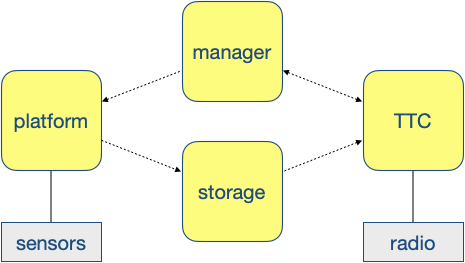
\includegraphics[width=.6\textwidth,keepaspectratio]{obdh.png}}
            \caption{OBDH system architecture.}
            \label{fig:obdh}
\end{figure}

\begin{itemize}
\item The {\tt platform} subsystem performs housekeeping functions on the satellite platform. It is expanded from the housekeeping component developed in the previous laboratory assignments in order to include an additional sensor. The list of variables that are monitored is now:
\begin{itemize}
\item OBC\_T : OBC temperature
\item OBC\_V : OBC voltage
\end{itemize}
The state of the platform is the set of values measured at a particular time, with a timestamp indicating the time at which they have been acquired. Mission time, a monotonic seconds count from the system start time, is used to this purpose.
\item The {\tt storage} subsystem keeps trace of the last N state values measured by the platform subsystem, where N is a configurable system parameter.
\item The {\tt TTC} system is in charge of all communications with the ground station. Its functionality includes:
\begin{itemize}
\item {\tt Telemetry} (TM) messages transmitted to ground, which may be of the following kinds:
\begin{itemize}
\item {\tt Basic} telemetry (Hello) messages, including the last measured values from all the sensors. These messages are periodically transmitted when the system is in idle mode (see below).
\item {\tt Housekeeping} messages include a more complete record with the last N stored values of the state. These messages are transmitted in response to a telecommand.
\item {\tt Mode} messages indicating the current operating mode of the system are transmitted after every mode change (see below).
\item {\tt Error} messages are occasionally sent to indicate some kinds of errors.
\end{itemize}
\item {\tt Telecommands} (TC) are messages received from ground, and can be of the following kinds:
\begin{itemize}
\item {\tt Open\_Link} messages are sent from the ground station in order to start a coverage period (see below).
\item {\tt Request\_HK} telecommands are used to request the OBDH system to send a housekeeping telemetry message.
\item {\tt Close\_Link} telecommands are sent by the ground station in order to close a coverage period and return to the idle mode (see below).
\item An {\tt error} TC value is signalled by the TTC subsystem when a message received from ground cannot be properly decoded as a valid TC.
\end{itemize}
\end{itemize}
\item The {\tt manager} subsystem carries out functions related to the operating mode of the system and the execution of telecommands. In this simplified OBDH system only two modes of operation are defined, related to the (simulated) visibility of the satellite from the ground station.
\begin{itemize}
\item {\tt Idle}. The system is this mode when the satellite is not visible from the ground station.
\item {\tt Coverage}. The system is in coverage mode when the satellite is visible from the ground station.
\end{itemize}
Mode changes are started from the TTC subsystem, according to the following protocol:
\item When in {\tt idle} mode, the OBDH system periodically transmits basic TM messages, and listens to telecommands from ground. When an open\_link TC is received, it requests the manager to switch to the coverage mode. No other kinds of telecommands are accepted in this mode.
\item When in {\tt coverage} mode, basic telemetry is not transmitted, and the TTC subsystem listens to telecommands from the ground station. The system switches back to idle mode when a close link TC is received or, alternatively, a maximum coverage time span has passed.
\end{itemize}

\section{System design}
The task structure of the system that has been designed in order to provide the above functionality is shown on figure~\ref{fig:obdh-task}.
\begin{figure}[h]
            \centering{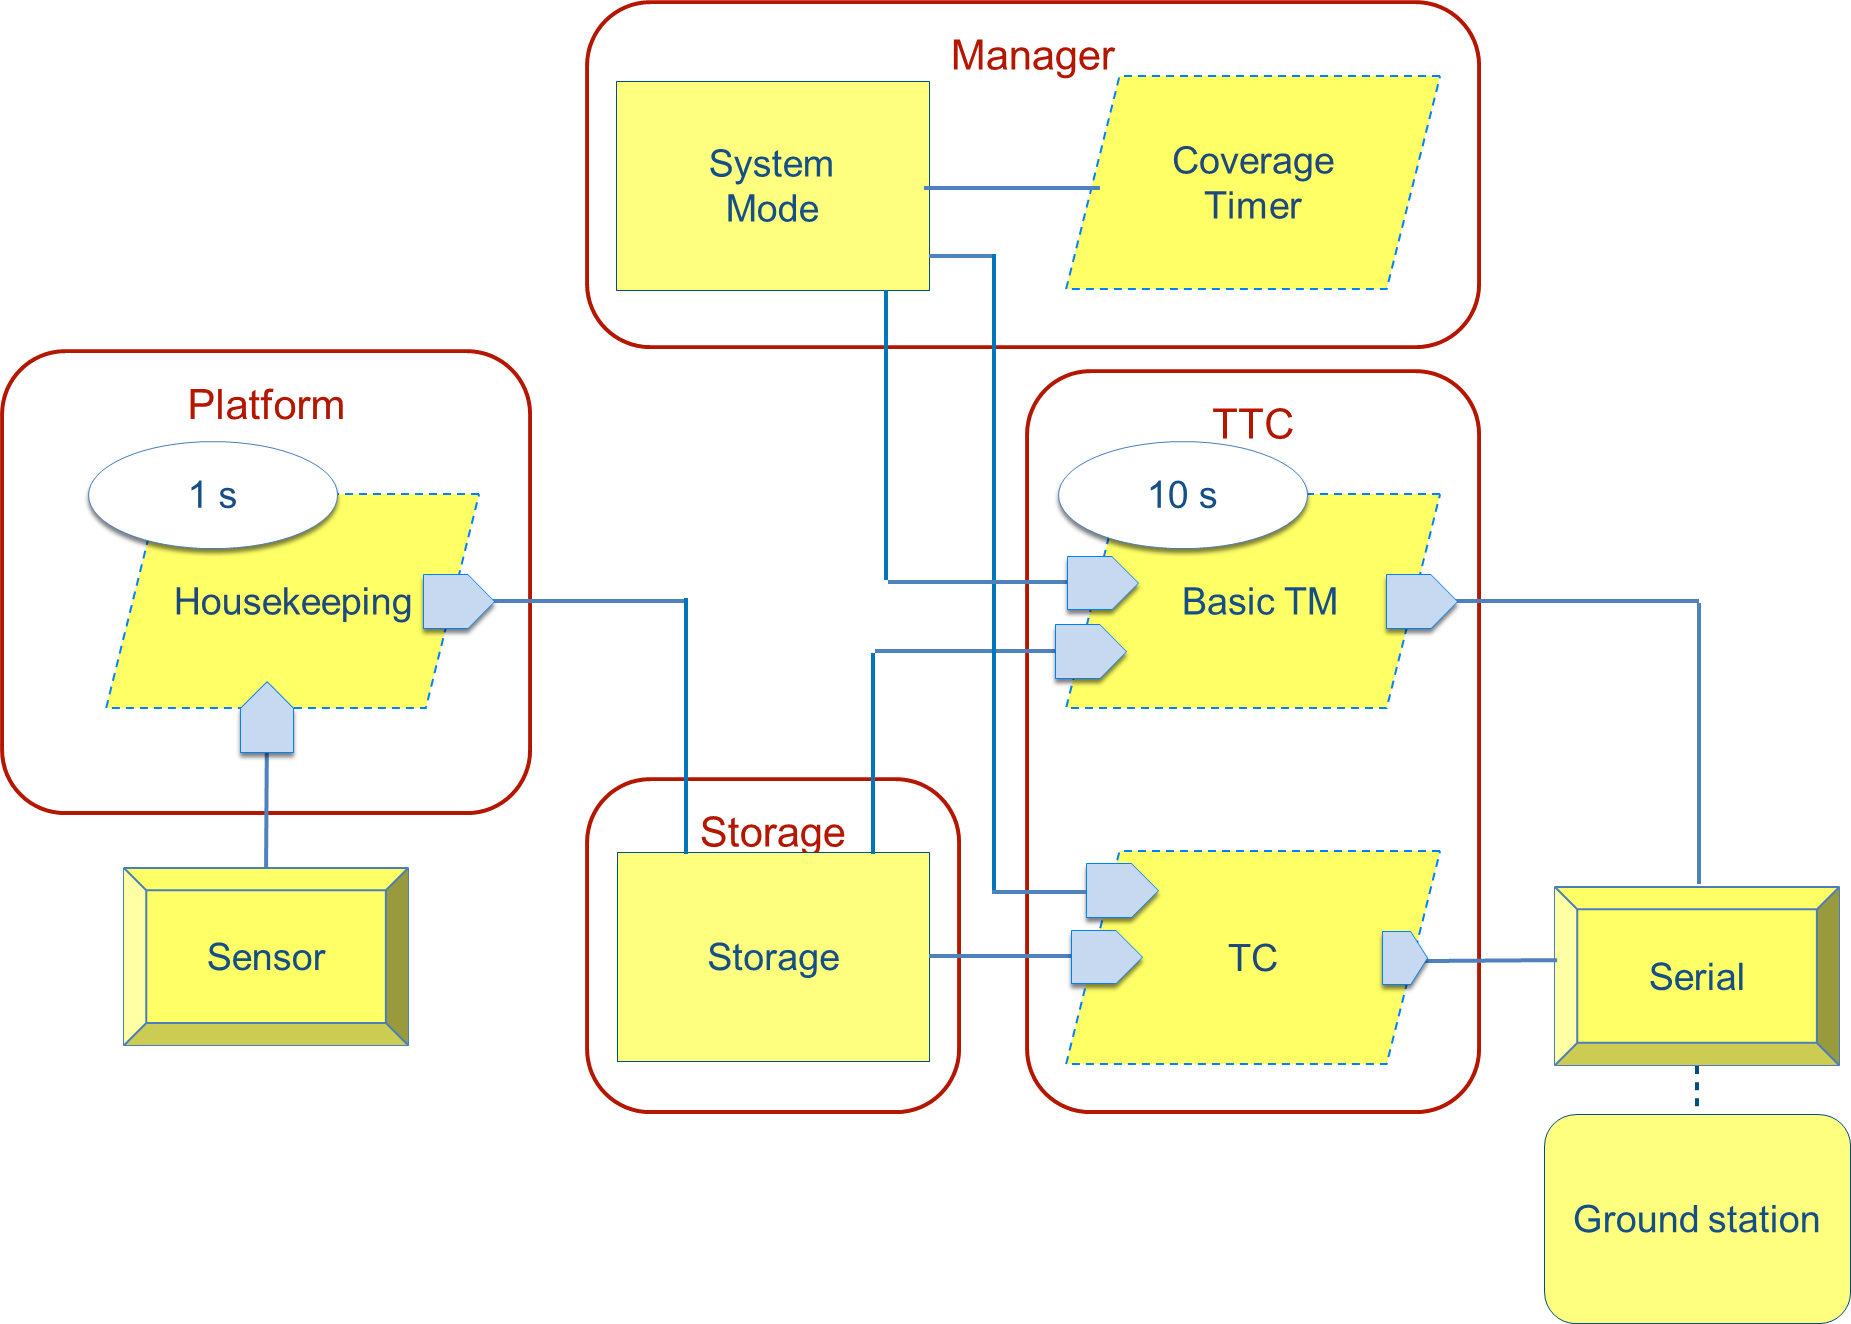
\includegraphics[width=\textwidth,keepaspectratio]{obdh-task.png}}
            \caption{OBDH system task structure.}
            \label{fig:obdh-task}
\end{figure}

\section{Real-time requirements}

The following real-time requirements are specified for the system:
\begin{itemize}
\item The {\tt Housekeeping} task executes with a period of 1 s and has a deadline of 100 ms.
\item The {\tt Basic\_TM} task executes with a period of 10 s and has a deadline of 500 ms.
\item The {\tt TC} task is sporadic, and is executed upon reception of a telecommand. The minimum separation of the event is 2 s, and the deadline is 1 s.
\item The {\tt Coverage\_Timer} task is sporadic with a minimum separation of 60 s and a deadline of 1 s.
\end{itemize}
Priorities are assigned in deadline-monotonic order, as shown in table~\ref{tb:obdh-requirements}. The {\tt Buffer} protected object, which is part of the {\tt Storage} implementation, is accessed by the {\tt Housekeeping}, {\tt Basic\_TM} and {\tt TC} tasks, and thus has a ceiling priority equal to the priority of the {\tt Housekeeping} task.

\begin{table}[htb]
\begin{center}
\begin{tabular}{|l|r|r|r|} \hline
Task & Period & Deadline & Priority\\ \hline
Housekeeping & 1.0 & 1.0 & 20 \\
Coverage\_Timer & 60.0 & 1.0 & 15 \\
Basic\_TM & 10.0 & 0.5 & 12 \\
TC & 1.0 & 1.0 & 10 \\
Storage buffer & - & - & 20 \\ \hline
\end{tabular}
\caption{OBDH real-time requirements.}
\label{tb:obdh-requirements}
\end{center}
\end{table}

\section{Download the code and study the implementation}


The implementation code, as initially provided to the students, can be downloaded from \url{https://github.com/STR-UPM/OBDH\_LABS}. Click on {\tt Clone} or {\tt download}, download a zip archive, unzip and move to your work directory. The code for the OBDH system is in the PROJECT/OBDH folder.

The implementation code reflects the task structure in figure~\ref{fig:obdh-task}.

\section{Compile and run.}

Open GPS and do the following:
\begin{enumerate}
\item Select {\tt Open} project on the welcome window. Navigate to the PROJECT/OBDH directory and open the {\tt obdh.gpr} project file.
\item Build the executable and load it into the board by clicking on the \hbox{
\includegraphics[width=1.5em]{buildandload.png}} symbol in the tool bar (or select {\tt Build} $\rightarrow$ {\tt Bareboard} $\rightarrow$ {\tt Flash to board} on the top menu).

The program will be compiled, and the executable will be loaded into the board flash memory. After that, the program starts to run on the board (check the blinking LEDs).
\item Connect the serial cable to a USB port on the host computer, if not already done, following the instructions in section~\ref{sc:serial} of this manual.

\item Identify the serial port name on the host computer and launch the remote terminal application as explained in section~\ref{sc:term}.The output shows all telemetry messages received from the board, including basic housekeeping
in idle mode and responses to telecommands (figure~\ref{fig:obdh-output}).
\end{enumerate}

\begin{figure}[h]
            \centering{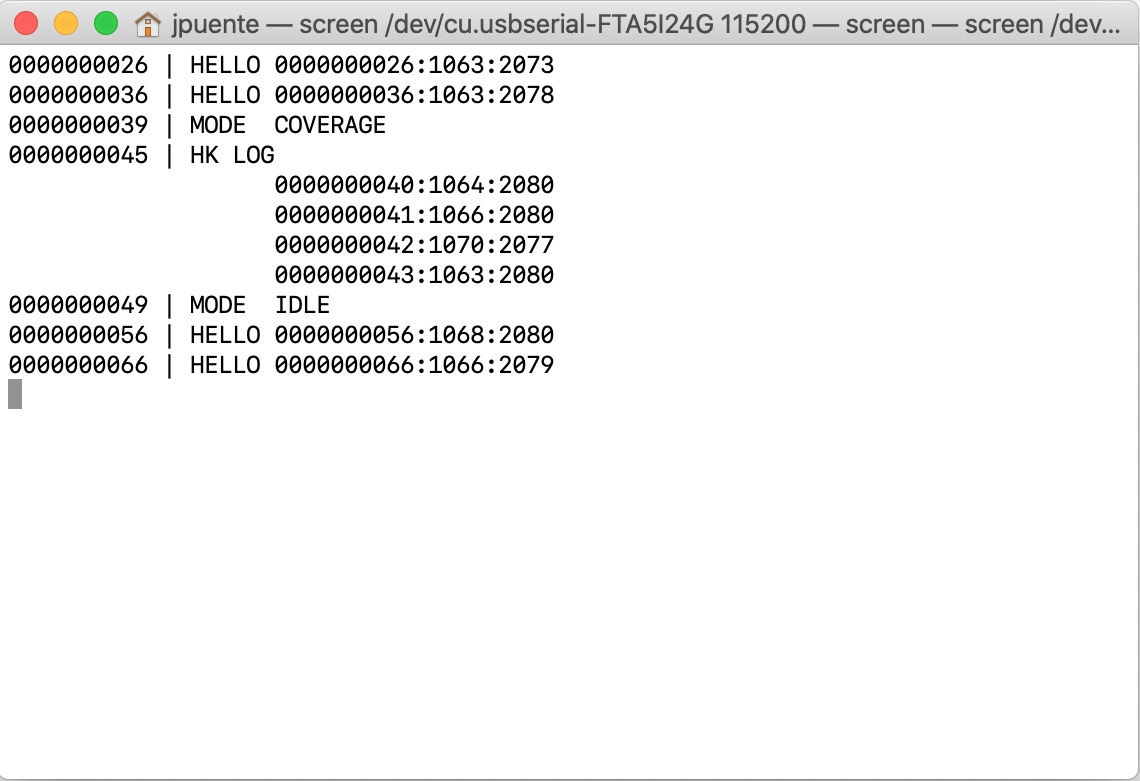
\includegraphics[width=0.6\textwidth,keepaspectratio]{obdh-output.png}}
            \caption{Sample telemetry messages received at the host terminal.}
            \label{fig:obdh-output}
\end{figure}

\section{Ground station}

The appearance of the output can be improved by using dedicated software. A simple example is the python script {\tt gs.py} located in PROJECT/GS directory. In order to use it, do the following:
\begin{enumerate}
\item Install Python in your system, if not already installed.
\item Install the {\tt pip} package manager if not already installed
\item Install the {\tt pySerial} module:
\begin{verbatim}
python -m pip install pyserial
\end{verbatim}
\item Edit the file {\tt gs.py} and set the serial port name on the host computer :
\begin{verbatim}
serial_port = 'COM4'
\end{verbatim}

\item Run the script from a terminal window, with the board connected to the host PC:
\begin{verbatim}
python gs.py
\end{verbatim}
\end{enumerate}
A sample of the telemetry messages received at the ground station is shown in figure~\ref{fig:gs-output}. The command ``exit'' terminates the execution of the ground station script.

\begin{figure}[h]
            \centering{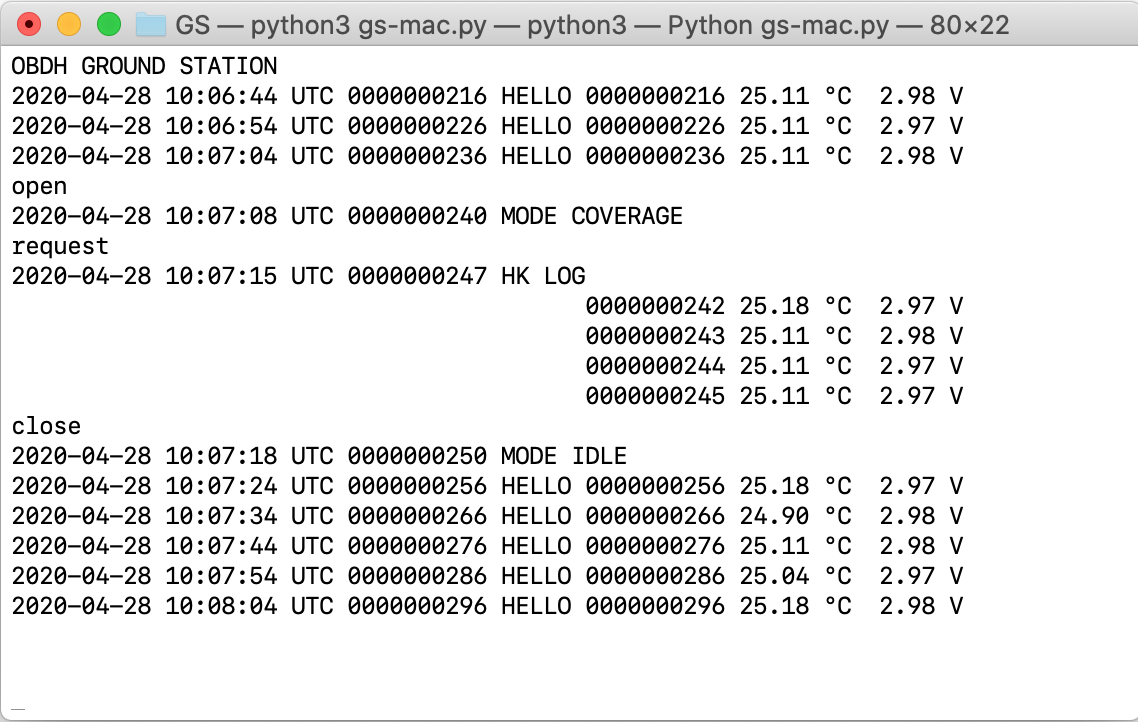
\includegraphics[width=0.6\textwidth,keepaspectratio]{gs-output.png}}
            \caption{Sample telemetry messages received at the GS script.}
            \label{fig:gs-output}
\end{figure}

